\documentclass[10pt,a4paper]{article}
\usepackage[utf8]{inputenc}
\usepackage{graphicx}
\author{Matthew Dittmer}
\title{MACFormatter: Hardware address format converter}
\begin{document}
\maketitle
\section*{Introduction}

The purpose of this application is to convert hardware
 addresses to colon delimited octets.  Hardware addresses, 
 or MAC(Media Access Control) addresses, are expressed in a 
 variety of forms.  These forms include two octets 
 delimited by colons, dashes, periods, and no delimiters at 
 all.  There are many use for one form in particular.  Two 
 octets separated by colons are expected input for a 
 variety of systems including wireless logs and access 
 control lists.

\section*{Usage}

The usage of this application is simple.  One can paste or 
type the hardware address in the the entry box and click 
"convert".  The converted address will appear at the bottom 
of the window.

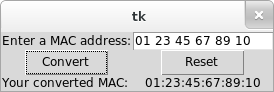
\includegraphics[scale=.5]{screenshot0.png}

In addition to being show at the bottom of the window in 
colon delmited form, the application will automatically 
copy the result to the clipboard to paste for use in 
another system.

\section*{Support}

To report bugs and provide feedback, please email 
dittmer.matthew@gmail.com

\section*{License}

The purpose of this application is to convert hardware 
addresses to colon delimited octets.
Copyright (C) 2013  Matthew Dittmer

This program is free software; you can redistribute it 
and/or modify it under the terms of the GNU General Public 
License as published by the Free Software Foundation;
either version 2 of the License, or (at your option) any 
later version.

This program is distributed in the hope that it will be 
useful, but WITHOUT ANY WARRANTY; without even the implied 
warranty of MERCHANTABILITY or FITNESS FOR A PARTICULAR 
PURPOSE.  See the GNU General Public License for more 
details.

You should have received a copy of the GNU General Public 
License along with this program; if not, write to the Free 
Software Foundation, Inc., 51 Franklin Street, Fifth Floor, 
Boston, MA  02110-1301, USA.

\end{document}
